\documentclass{beamer}

% does not look nice, try deleting the line with the fontenc.
\usepackage[english]{babel}
\usepackage{amsmath}
\usepackage[latin1]{inputenc}
\usepackage{units}
\usepackage{colortbl}
\usepackage{multimedia}
\usepackage{bm}
\usepackage{subcaption}
\usepackage{algorithm2e}
\usepackage{algorithmic}

\mode<presentation>
{
  \usetheme{Boadilla}
  \useoutertheme{infolines}
  \setbeamercovered{transparent} 
}
	

\title[Neural System Identification]{\textsc{Model Structures and Fitting Criteria for System Identification with Neural Networks}}


\author[]{Marco Forgione, Dario Piga}

\institute[IDSIA]{IDSIA Dalle Molle Institute for Artificial Intelligence SUPSI-USI, Lugano, Switzerland} 


\date[AICT 2020]{14th IEEE International Conference on Application of Information and Communication Technologies}


\subject{System Identification, Deep Learning, Machine Learning, Regularization}


%% MATH DEFINITIONS %%
\newcommand{\So}{S_o} % true system
\newcommand{\hidden}[1]{\overline{#1}}
\newcommand{\nsamp}{N}
\newcommand{\Yid}{Y}
\newcommand{\Uid}{U}
\newcommand{\Did}{{\mathcal{D}}}
\newcommand{\tens}[1]{\bm{#1}}

\newcommand{\batchsize}{q}
\newcommand{\seqlen}{m}
\newcommand{\nin}{n_u} 
\newcommand{\ny}{n_y} 
\newcommand{\nx}{n_x}

\newcommand{\NN}{\mathcal{N}} % a feedforward neural network

\newcommand{\norm}[1]{\left \lVert #1 \right \rVert}
\DeclareMathOperator*\argmin{arg \, min}

\definecolor{darkgreen}{RGB}{20,150,50}

\begin{document}

\begin{frame}
  \titlepage
\end{frame}
\begin{frame}{Motivations}
%Neural Networks are very expressive models structures, but oftel lack physical interpretability.\\

Neural Networks are commonly used to model dynamical systems. However, they seldom exploit
available \structure{a priori} knowledge.\\
%\vskip 1em
%Training RNNs requires a \structure{sequential simulation} through the training time steps, which can be slow. 
%How to parallelize the training procedure?
\vskip 2em
\pause
In this work:
\begin{itemize}
\item We present \structure{tailor-made model structures} for system identification with Neural Networks 
\item We develop \structure{efficient algorithms} to fit these model structures to data. 
\end{itemize}
\end{frame}

\begin{frame}{Settings}
The \structure{data-generating system} $\So$ is assumed to have the discrete-time  state-space representation:
\begin{equation*}
\begin{split}
 x_{k+1} &= f(x_{k}, u_{k}) \\
 y^{\text o}_k     &= g(x_k)\\
 y_k &= y^{\text o}_k + e_k
\end{split}
\end{equation*}
%\pause
\vskip 1em
\structure{Training dataset} $\Did$ consisting of $\nsamp$ input samples $\Uid = \{u_{0},\;u_{1},\dots,\;u_{\nsamp-1}\}$ and output samples  $\Yid = \{y_{0},\;y_{1},\dots,\;y_{\nsamp-1}\}$ available.
\vskip 1em
%\pause
\structure{Objective}: estimate a dynamical model of $\So$.
\end{frame}

\begin{frame}{Neural Dynamical Models}{}
A very \structure{generic} neural model structure:
%\begin{align*}
% x_{k+1} &= \NN_f(x, u;\;\theta)\\
%    y_k  &= \NN_u(x; \theta)
%\end{align*}
\begin{align*}
 x_{k+1} &= \NN_f(x_k, u_k;\;\theta)\\
    y_k  &= \NN_g(x_k; \theta)
\end{align*}

where $\NN_f$, $\NN_g$ are feed-forward neural networks.
Can be  \structure{specialized}:
\pause 
\begin{itemize}
 \item Linear approximation available $\Rightarrow$
\begin{equation*}
\begin{split}
 x_{k+1} &= A x_k + B u_k + \NN_f(x_{k}, u_{k}; \theta)\\
 y_k     &= C x_k + \NN_g(x_{k}, u_{k}; \theta)
 \end{split}
\end{equation*}
 \pause
  \item State fully observed $\Rightarrow$ %$\NN_g = I$
\begin{align*}
 x_{k+1} &= \NN_f(x_k, u_k;\;\theta)\\
    y_k  &= x_k
\end{align*}
  %  \pause
%  \item Mechanical system, 1 DoF, measured position $\Rightarrow$
% \begin{equation*}
%  \begin{bmatrix}
%     \dot p   \\ 
%     \dot v \\
%   \end{bmatrix} = 
% %\dot x = 
%   \begin{bmatrix}
%    v \\
%    \NN_f(p, v, u; \theta)
%   \end{bmatrix}, \qquad
% 	y = p
% \end{equation*}

%\pause
%\item  No information $\Rightarrow$ neural \structure{IO structure}
%\begin{equation*}
% y_{k} = \NN_{\rm IO}(y_{k-1}, y_{k-2}\dots, y_{k-n_a},  u_{k-1},  u_{k-2}, \dots, u_{k-n_b}; \theta)
%\end{equation*}
 \end{itemize}
\end{frame}

\begin{frame}{Neural Dynamical Models}{Physics-inspired model structures}
\vskip 1em
Two-tank system, input=flow $u$ in upper tank, output=lower tank level $x_2$.
\begin{columns}
 \column{.6\textwidth}
 \begin{itemize}
  \item The system has two states: $x_1$ and $x_2$
  \item The state $x_1$ does not depend on $x_2$
  \item The state $x_2$ does not depend directly on $u$
  \item The state $x_2$ is observed
  \end{itemize}
 \column{.3\textwidth}
 \begin{center}
 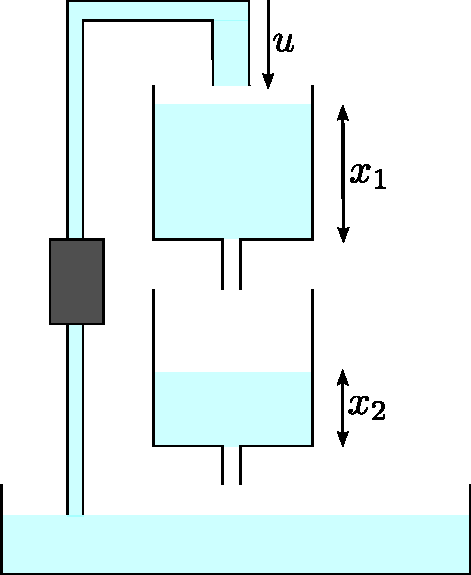
\includegraphics[width=.8\textwidth]{img/CTS/CTS_scheme.pdf}
 % CTS_scheme.pdf: 0x0 px, 300dpi, 0.00x0.00 cm, bb=
\end{center}
\end{columns}
\pause
\vskip 2em
The observations above lead to the neural \structure{physics-inspired} model structure
\begin{align*}
 \dot x_1 &= \NN_{1}(x_1, u)\\
 \dot x_2 &= \NN_{2}(x_1, x_2)\\
 y        &= x_2
\end{align*}

\end{frame}

\begin{frame}{Training Neural Dynamical Models}
% The \structure{naive} 1-step prediction is constructed through 
 In principle, \structure{simulation error minimization} is a valid strategy:
 \begin{equation*}
  \theta^o = \arg \min_{\theta, \hat x_0} \sum_{k=0}^{\nsamp-1} \norm{\hat y_k(\theta, \hat x_0) - y_k}^2
 \end{equation*}
 where
 \begin{equation*}
 \begin{split}
  \hat x_{k+1} &= \NN_f(\hat x_k, u_k;\;\theta)\\
  \hat{y}_k &= \NN_g(\hat x_k;\;\theta)
  \end{split}
 \end{equation*}
 for $k=0,1,\dots,\nsamp-1$.\\
\pause
\vskip .5em
 However, it is not convenient from a computational perspective:
 \begin{itemize}
  \item Simulation is \structure{not parallelizable}. Several neural network evaluations have to be performed \structure{sequentially}.
  \item \structure{Back-propagation cost} increases with the sequence length
 \end{itemize}
 \pause
 \vskip .5em
 In this work, we minimize instead the simulation error over \structure{batches} of $\batchsize$  \structure{subsequences}, each one of length $\seqlen \ll N$.
\end{frame}


% \begin{frame}{Training Neural Dynamical Models}
% We perform \structure{minibatch training} on $\batchsize$ subsequence of length $\seqlen$.\\
% \vskip 1em
% {for} each iteration of gradient-based optimization:
% \begin{enumerate}
% \item \textbf{extract} batch start index vector $s \in \mathbb{N}^\batchsize$
% \item \textbf{define} from $\Did$:
% \begin{itemize}
% \item input tensor $\tens {y} \in \mathbb{R}^{\batchsize \times \seqlen \times \ny}\qquad$ where $\tens{y}_{j,t} = Y_{s_{j}+t}$ 
% \item output tensor $\tens {u} \in \mathbb{R}^{\batchsize \times \seqlen \times \nin}\qquad$ 
% where $\tens{u}_{j,t} = U_{s_{j}+t}$ 
% \end{itemize}
% \pause
% \item \textbf{simulate} $\hat {\tens{y}}_{j,t}\qquad$ for $j=0,\dots,\batchsize\!-\!1$ and $t=0,\dots,\seqlen\!-\!1$.
% \begin{align*} 
%     \hat {\tens{x}}_{j, t+1} &= \hat {\tens x}_{j, t} + \NN_f(\hat {\tens x}_{j, t}, u_j, t)\\
% 	\hat {\tens{y}}_{j,t}  &= \NN_g(\hat {\tens x}_{j, t})
% \end{align*} 
% \vskip -2em
% \pause
%   \item \textbf{compute} the fitting loss
% $J(\theta) = \norm{\hat{\tens{y}}(\theta) - {{\tens{y}}}}^2
% $
% \pause
% \item \textbf{perform} gradient-based step (back-propagation) to minimize the cost
% \end{enumerate}
% \pause
% \vskip 1em
% Problem: what is the initial state $\tens{x}_{:,0}$ for simulation?
% \end{frame}

\begin{frame}{Training Neural Dynamical Models}
for each iteration of \structure{gradient-based} optimization:
\begin{figure}
\centering
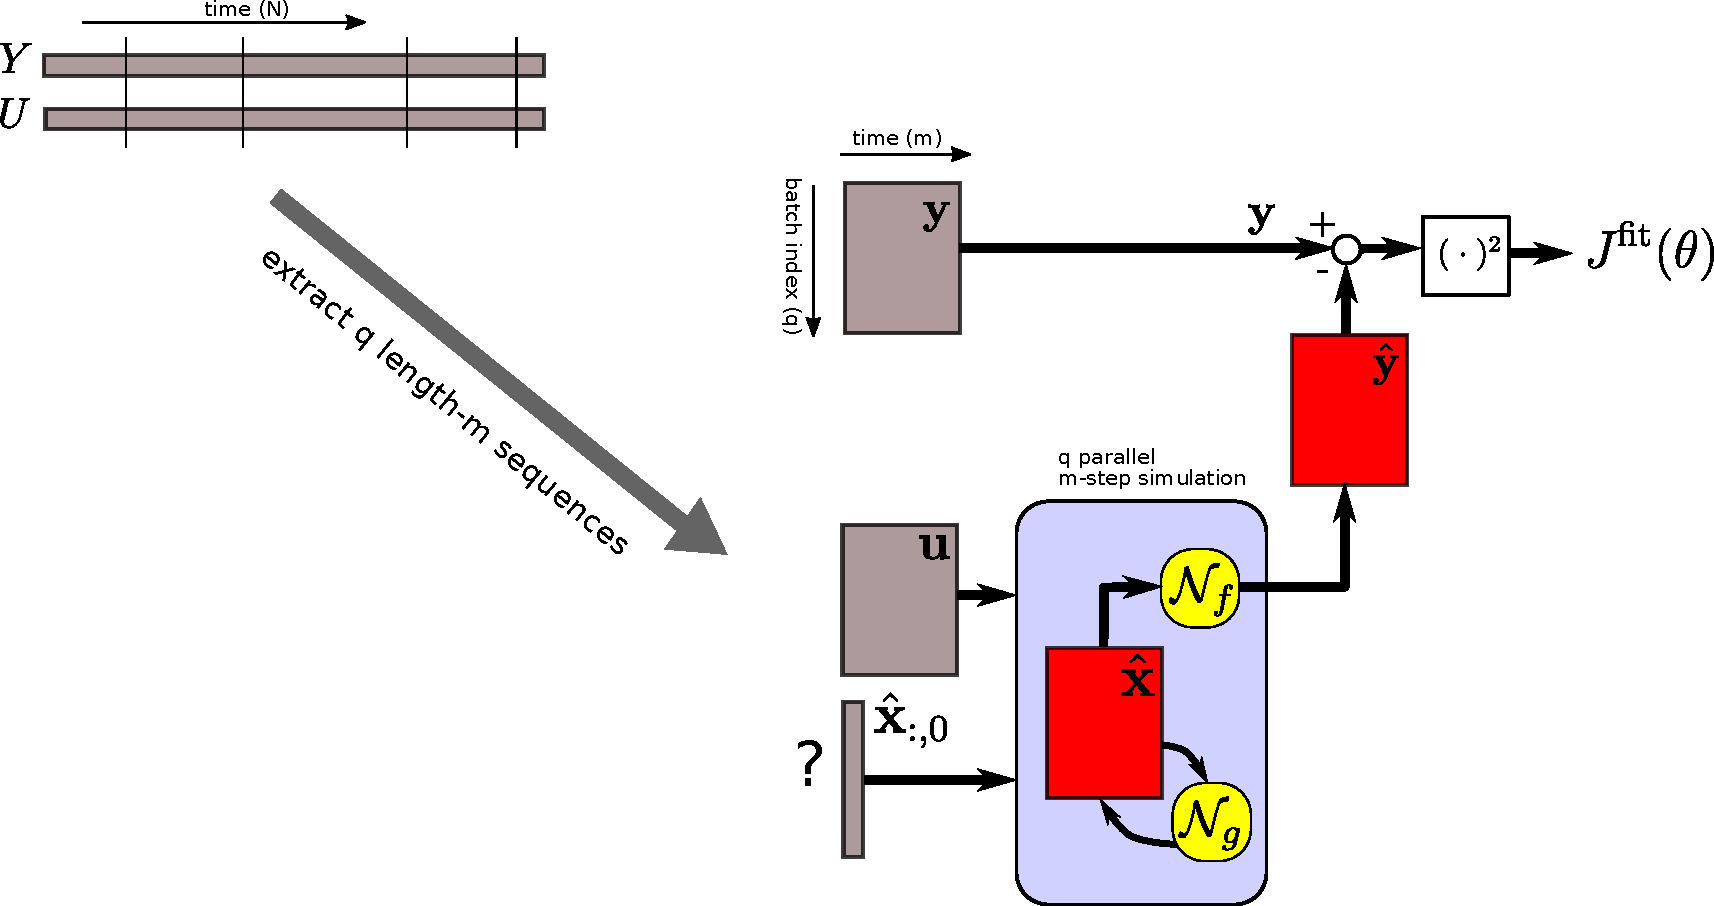
\includegraphics[width=.8\textwidth]{img/scheme/scheme_multistep_plain.pdf}
\end{figure}
\pause
Problem: how do we choose $\hat {\tens{x}}_{:, 0}$, the initial state for each batch? \\
We do not know it, but we need it to initialize all simulations.
\end{frame}

\begin{frame}{Training Neural Dynamical Models}
We consider the unknown state sequence $\hidden{X}$ as an \structure{optimization variable}.\\
We sample from $\hidden{X}$ to obtain the initial state for simulation in each batch. 
 \begin{figure}
\centering
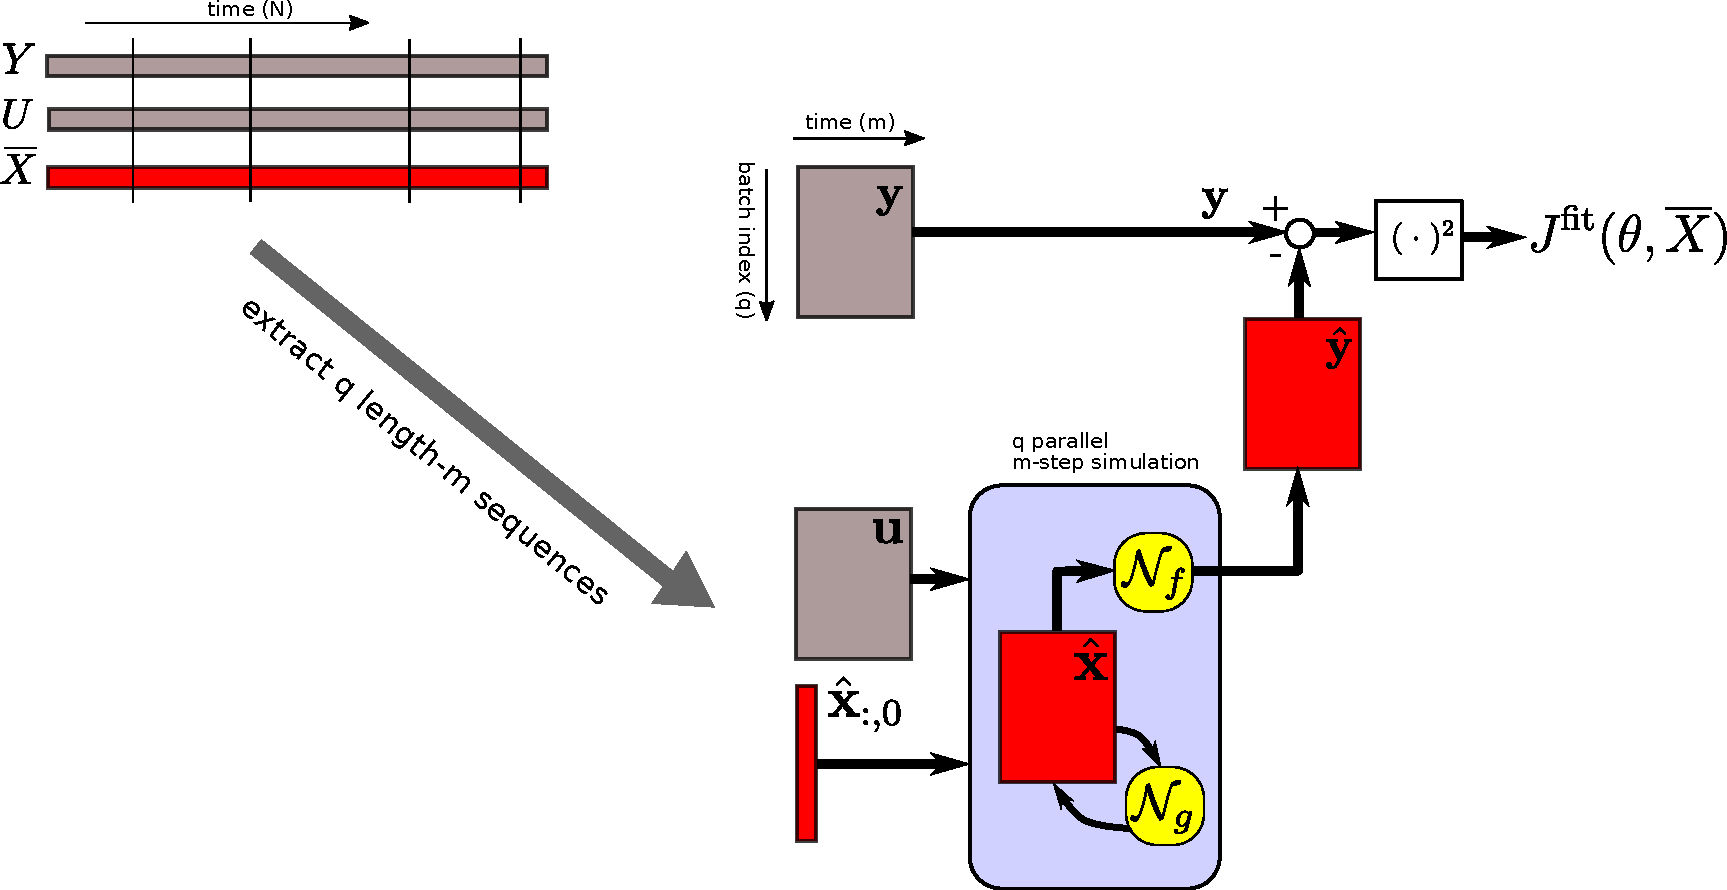
\includegraphics[width=.8\textwidth]{img/scheme/scheme_multistep_state_est.pdf}
\end{figure}
%\pause
$J^{\rm fit}$ is now a function of both $\theta$ and $\hidden{X}$. We optimize w.r.t. both!
\end{frame}

\begin{frame}{Training Neural Dynamical Models}
The hidden state sequence $\hidden{X}$ should also satisfy the identified dynamics!
We enforce this by adding a \structure{regularization term} in the cost function.
 \begin{figure}
\centering
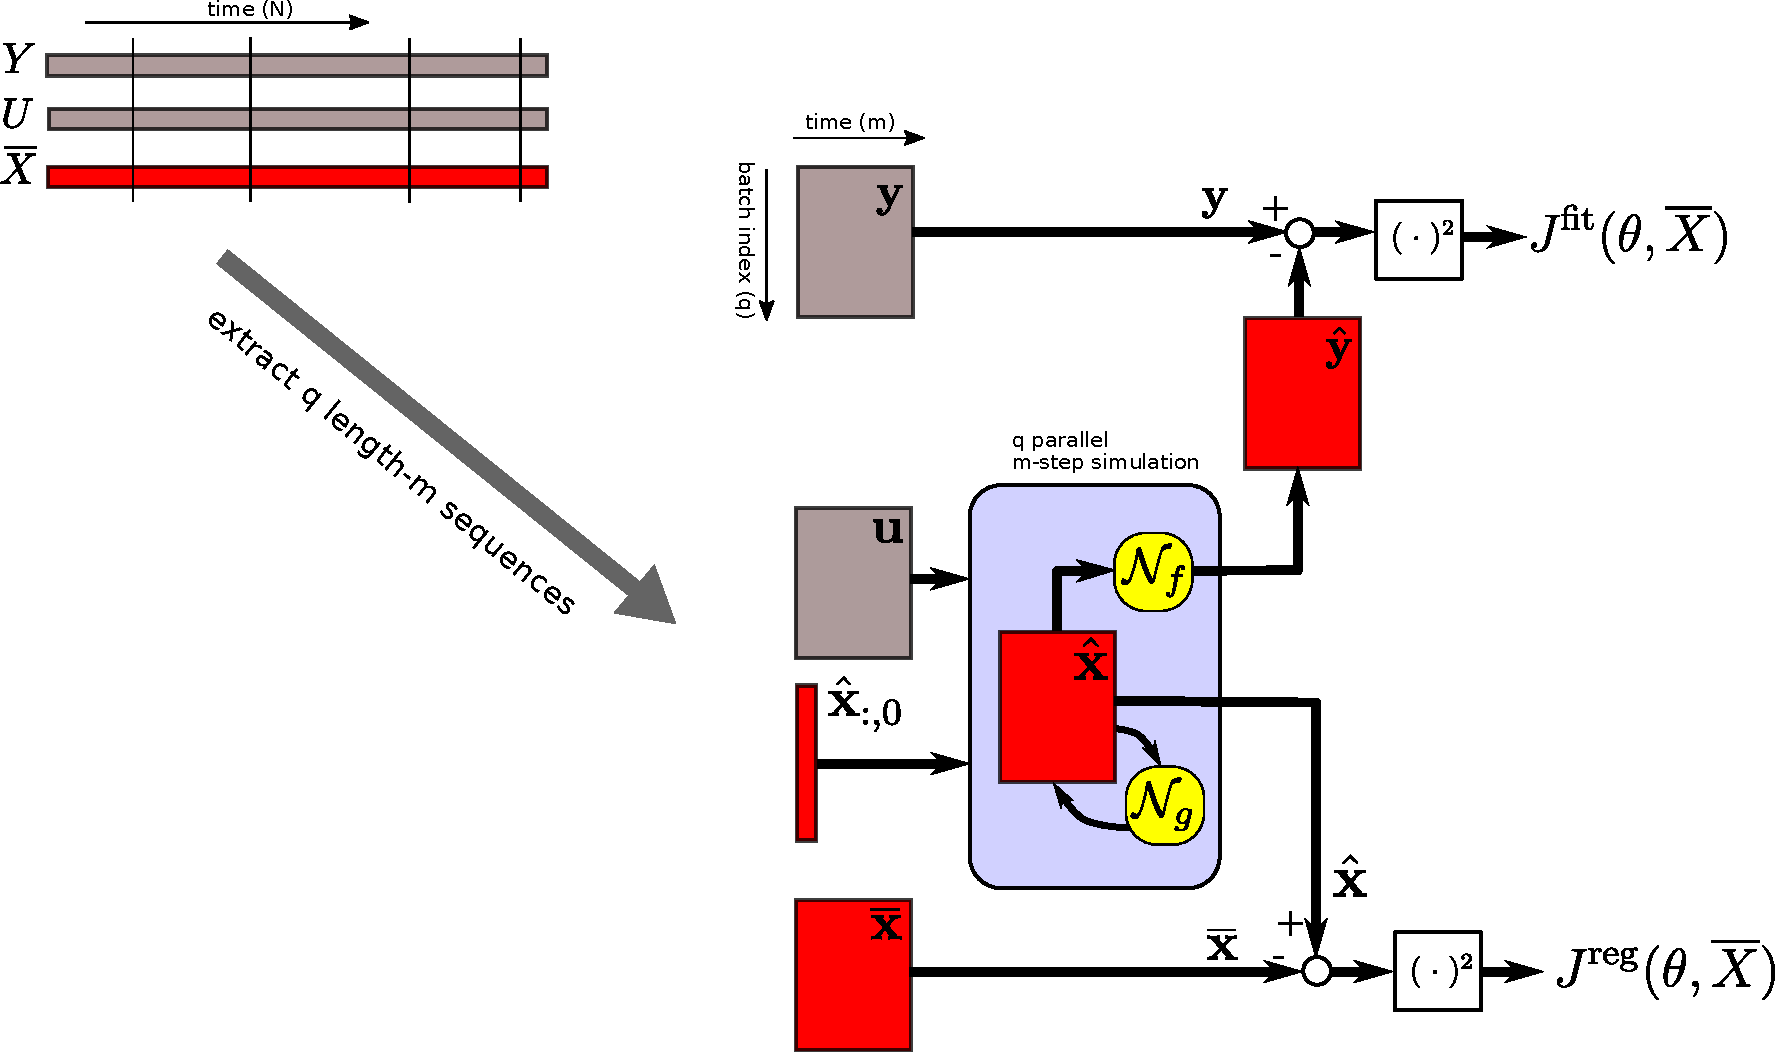
\includegraphics[width=.8\textwidth]{img/scheme/scheme_multistep_with_reg.pdf}
\end{figure}
%\pause
We minimize a \structure{weighted sum} of $J^{\rm fit}$ and $J^{\rm reg}$ w.r.t. both $\theta$ and $\hidden{X}$.
\end{frame}

% \begin{frame}{Training Neural Dynamical Models}{}
%  {for} each iteration of gradient-based optimization:
%  \begin{enumerate}
% \item \textbf{extract} batch start index vector $s \in \mathbb{N}^\batchsize$
% \item \textbf{define} from $\Did$:
% \begin{itemize}
% \item input tensor $\tens {y} \in \mathbb{R}^{\batchsize \times \seqlen \times \ny}\qquad\qquad$ where $\tens{y}_{j,t} = Y_{s_{j}+t}$ 
% \item output tensor $\tens {u} \in \mathbb{R}^{\batchsize \times \seqlen \times \nin}\qquad\;\;\;\;\;$ 
% where $\tens{u}_{j,t} = U_{s_{j}+t}$
% \item hidden state tensor $\hidden{\tens {x}} \in \mathbb{R}^{\batchsize \times \seqlen \times \nx}\;\;\;\;$ where 
% $\hidden{\tens{x}}_{j,t} = \hidden{X}_{s_{j}+t}$ 
% \item initial condition $\hat{\tens{x}}_{:,0}\qquad \qquad \qquad\;\;\;$ where 
% $\hat{\tens{x}}_{j,0}= \hidden{x}_{s_j}$
% \end{itemize}
% \pause
% \item \textbf{simulate} $\hat {\tens{y}}_{j,t}^{\mathrm{sim}}$
% \begin{align*} 
%     \hat {\tens{x}}_{j, t+1} &= \hat {\tens x}_{j, t} + \NN_f(\hat {\tens x}_{j, t}, u_j, t)\\
% 	\hat {\tens{y}}_{j,t}  &= \NN_g(\hat {\tens x}_{j, t})
% \end{align*} 
% \vskip -.5em
% \pause
% \vskip -.5em
%   \item \textbf{compute} the loss
% $J(\theta) = \norm{\hat{\tens{y}} - {{\tens{y}}}}^2 + \alpha \norm{\hat{\tens{x}} - {{\hidden{\tens{x}}}} }^2
% $
% \pause
% \item \textbf{perform} gradient-based step (back-propagation) to minimize the cost
% \end{enumerate}
% \end{frame}



\begin{frame}{Simulation example}{RLC circuit}
 We consider a nonliner \structure{RLC circuit}:
 \begin{columns}
 \column{.5\textwidth}
\footnotesize
 \begin{equation*}
\begin{bmatrix}
\dot v_C\\
\dot i_L
\end{bmatrix} = 
\begin{bmatrix}
  0           & \tfrac{1}{C}\\
 \tfrac{-1}{L(i_L)} & \tfrac{-R}{L(i_L)}\\
\end{bmatrix}
\begin{bmatrix}
v_C\\
i_L
\end{bmatrix} +
\begin{bmatrix}
0\\
\tfrac{1}{L(i_L)}
\end{bmatrix} 
v_{in}
\end{equation*}
 \column{.5\textwidth}
 \vskip -2em
\begin{figure}
\centering
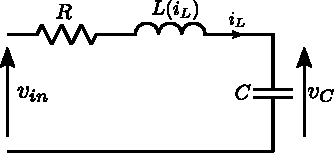
\includegraphics[width=.7\linewidth]{img/RLC/RLC.pdf}
\end{figure}
\end{columns}
\vskip 1em
with %$R = 3~\Omega$, $C=270~\text{nF}$, and 
\structure{nonlinear inductance} $L(i_L)$
\vskip -1em
\begin{columns}
 \column{.5\textwidth}
\footnotesize
 \begin{equation*}
 L(i_L) = L_0\bigg[\bigg(\frac{0.9}{\pi}\!\arctan\!\big(-\!5(|i_L|\!-\!5\big)+0.5\bigg) + 0.1 \bigg]%~\text{H}
\end{equation*}
 \column{.5\textwidth}
\begin{figure}
\centering
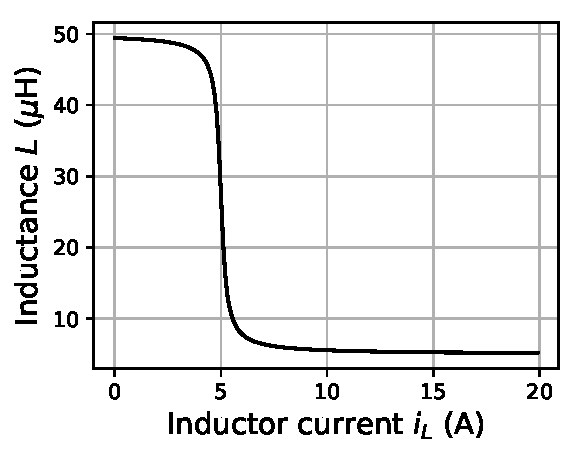
\includegraphics[width=.5\linewidth]{img/RLC/RLC_characteristics.pdf}
\end{figure}
 \end{columns}
%\pause
\vskip 0.5em
Input: voltage $v_{in}$.  Output: voltage $v_C$, current $i_L$. \text{SNR}=20 \\%Datasets:
%\begin{itemize}
%\item identification: $N\!=\!4000$, filtered w.n. $\sigma_v\!=\!80~V$, $B_v\!=\!150~kHz$
%\item validation: $N\!=\!4000$,  $v_{in}$ filtered w.n. $\sigma_v\!=\!60~V$, $B_v\!=\!%200~kHz$
%\end{itemize}
\pause
\vskip .5em
Neural model structure: \structure{fully observed state}
\begin{equation*}
\begin{split}
 x_{k+1} &= \NN_f(x_{k}, u_{k}; \theta)\\
 y_k     &= x_k
 \end{split}
\end{equation*}
\end{frame}

% \begin{frame}{Simulation example}{RLC circuit}
% Results \structure{in simulation} on the test dataset. Training with:
% \vskip 1em
%  \begin{columns}
%   \column{.5\textwidth}
%   \centering
%   1-step prediction, $\text{SNR}=\infty$
%   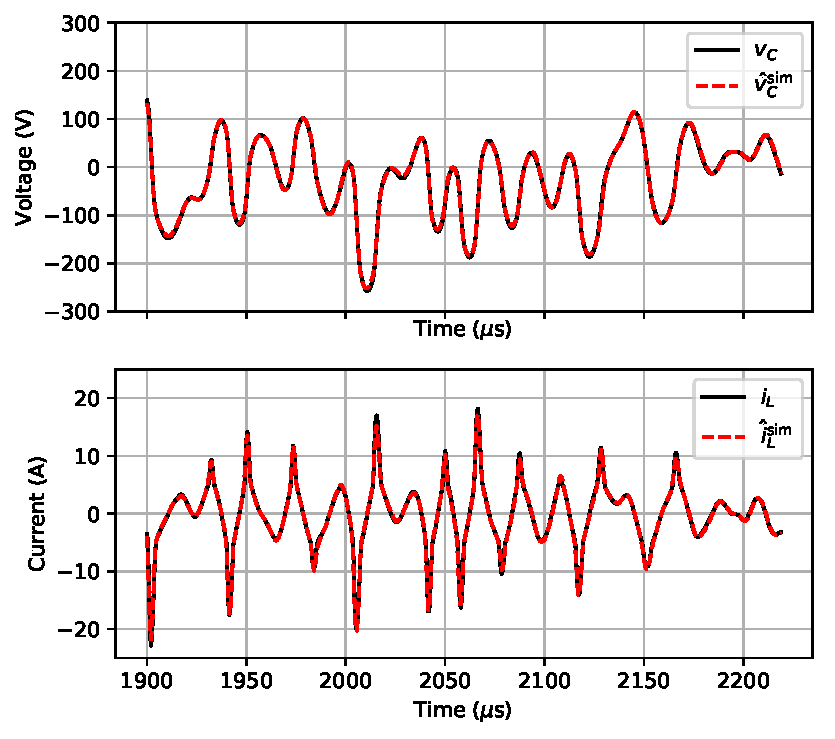
\includegraphics[width=\textwidth]{img/RLC/RLC_SS_val_64step_noise.pdf}
%   train time: 90~s
%   \column{.5\textwidth}
%     \centering
%   1-step prediction, $\text{SNR}=20~\text{dB}$
%   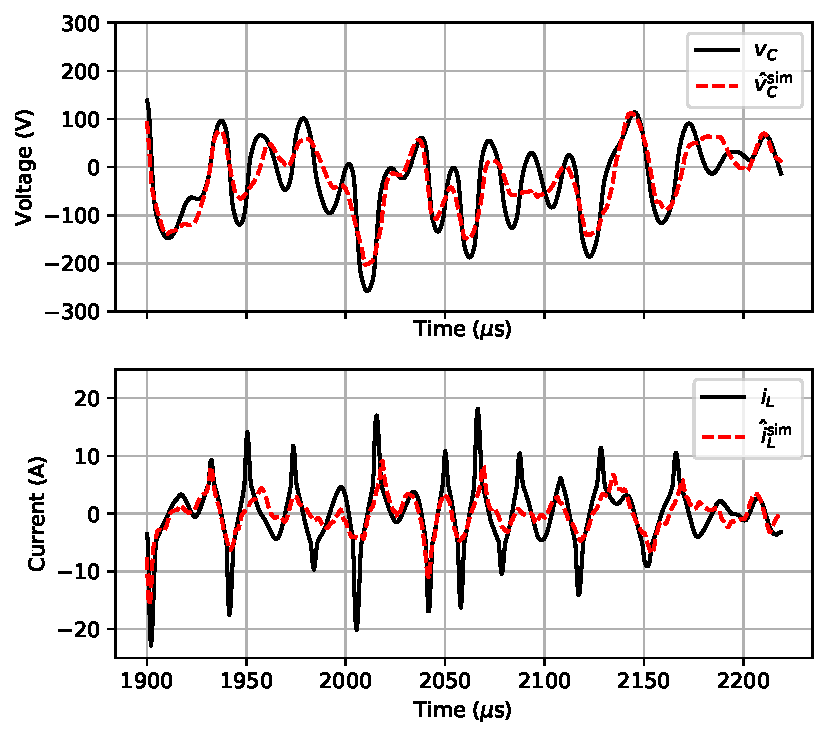
\includegraphics[width=\textwidth]{img/RLC/RLC_SS_val_1step_noise.pdf}
%     train time: 90~s
%   \end{columns}
% \end{frame}


\begin{frame}{Numerical example}{RLC circuit}
Results \structure{in simulation} on the test dataset. Training with:
\vskip 1em
\begin{columns}
  \column{.5\textwidth}
  \centering
  $q=62$ sequences of length $m=64$ %, %$\text{SNR}=20~\text{dB}$
  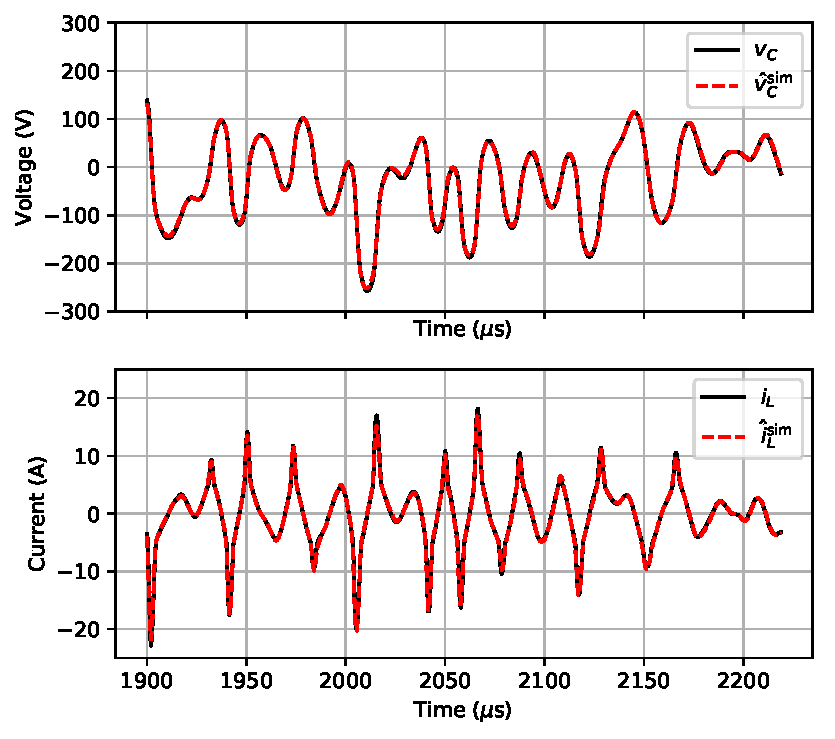
\includegraphics[width=\textwidth]{img/RLC/RLC_SS_val_64step_noise.pdf}
  train time: 320~s
  \column{.5\textwidth}
    \centering
  simulation error minimization\\ %$\text{SNR}=20~\text{dB}$
  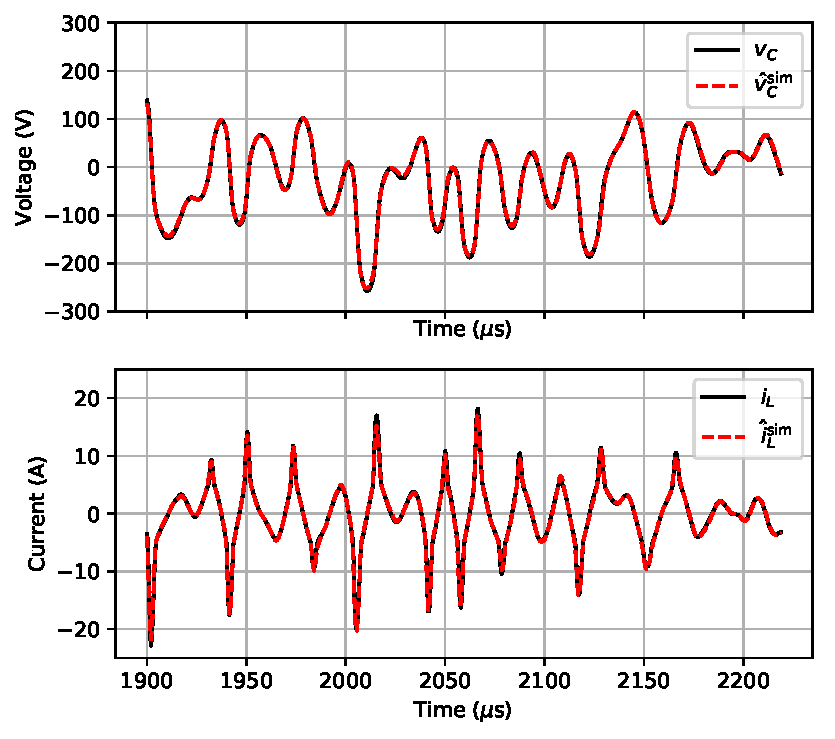
\includegraphics[width=\textwidth]{img/RLC/RLC_SS_val_64step_noise.pdf}
  \alert{train time: 7000~s}
  \end{columns}
\end{frame}

\begin{frame}{Numerical example}{Cascaded Tank System}
Dataset with \structure{real measurements} from \url{www.nonlinearbenchmark.org}
%\vskip 1em
\begin{columns}
 \column{.60\textwidth}
% System equations (no overflow)
% \begin{equation*}
%  \begin{split}
%   \dot x_1 &= -k_1\sqrt{x_1} + k_4 u\\
%   \dot x_2 &= k_2 \sqrt{x_1} - k_3 \sqrt{x_2}\\
%   y  &= x_2
%  \end{split}
% \end{equation*}
\begin{figure}
\centering
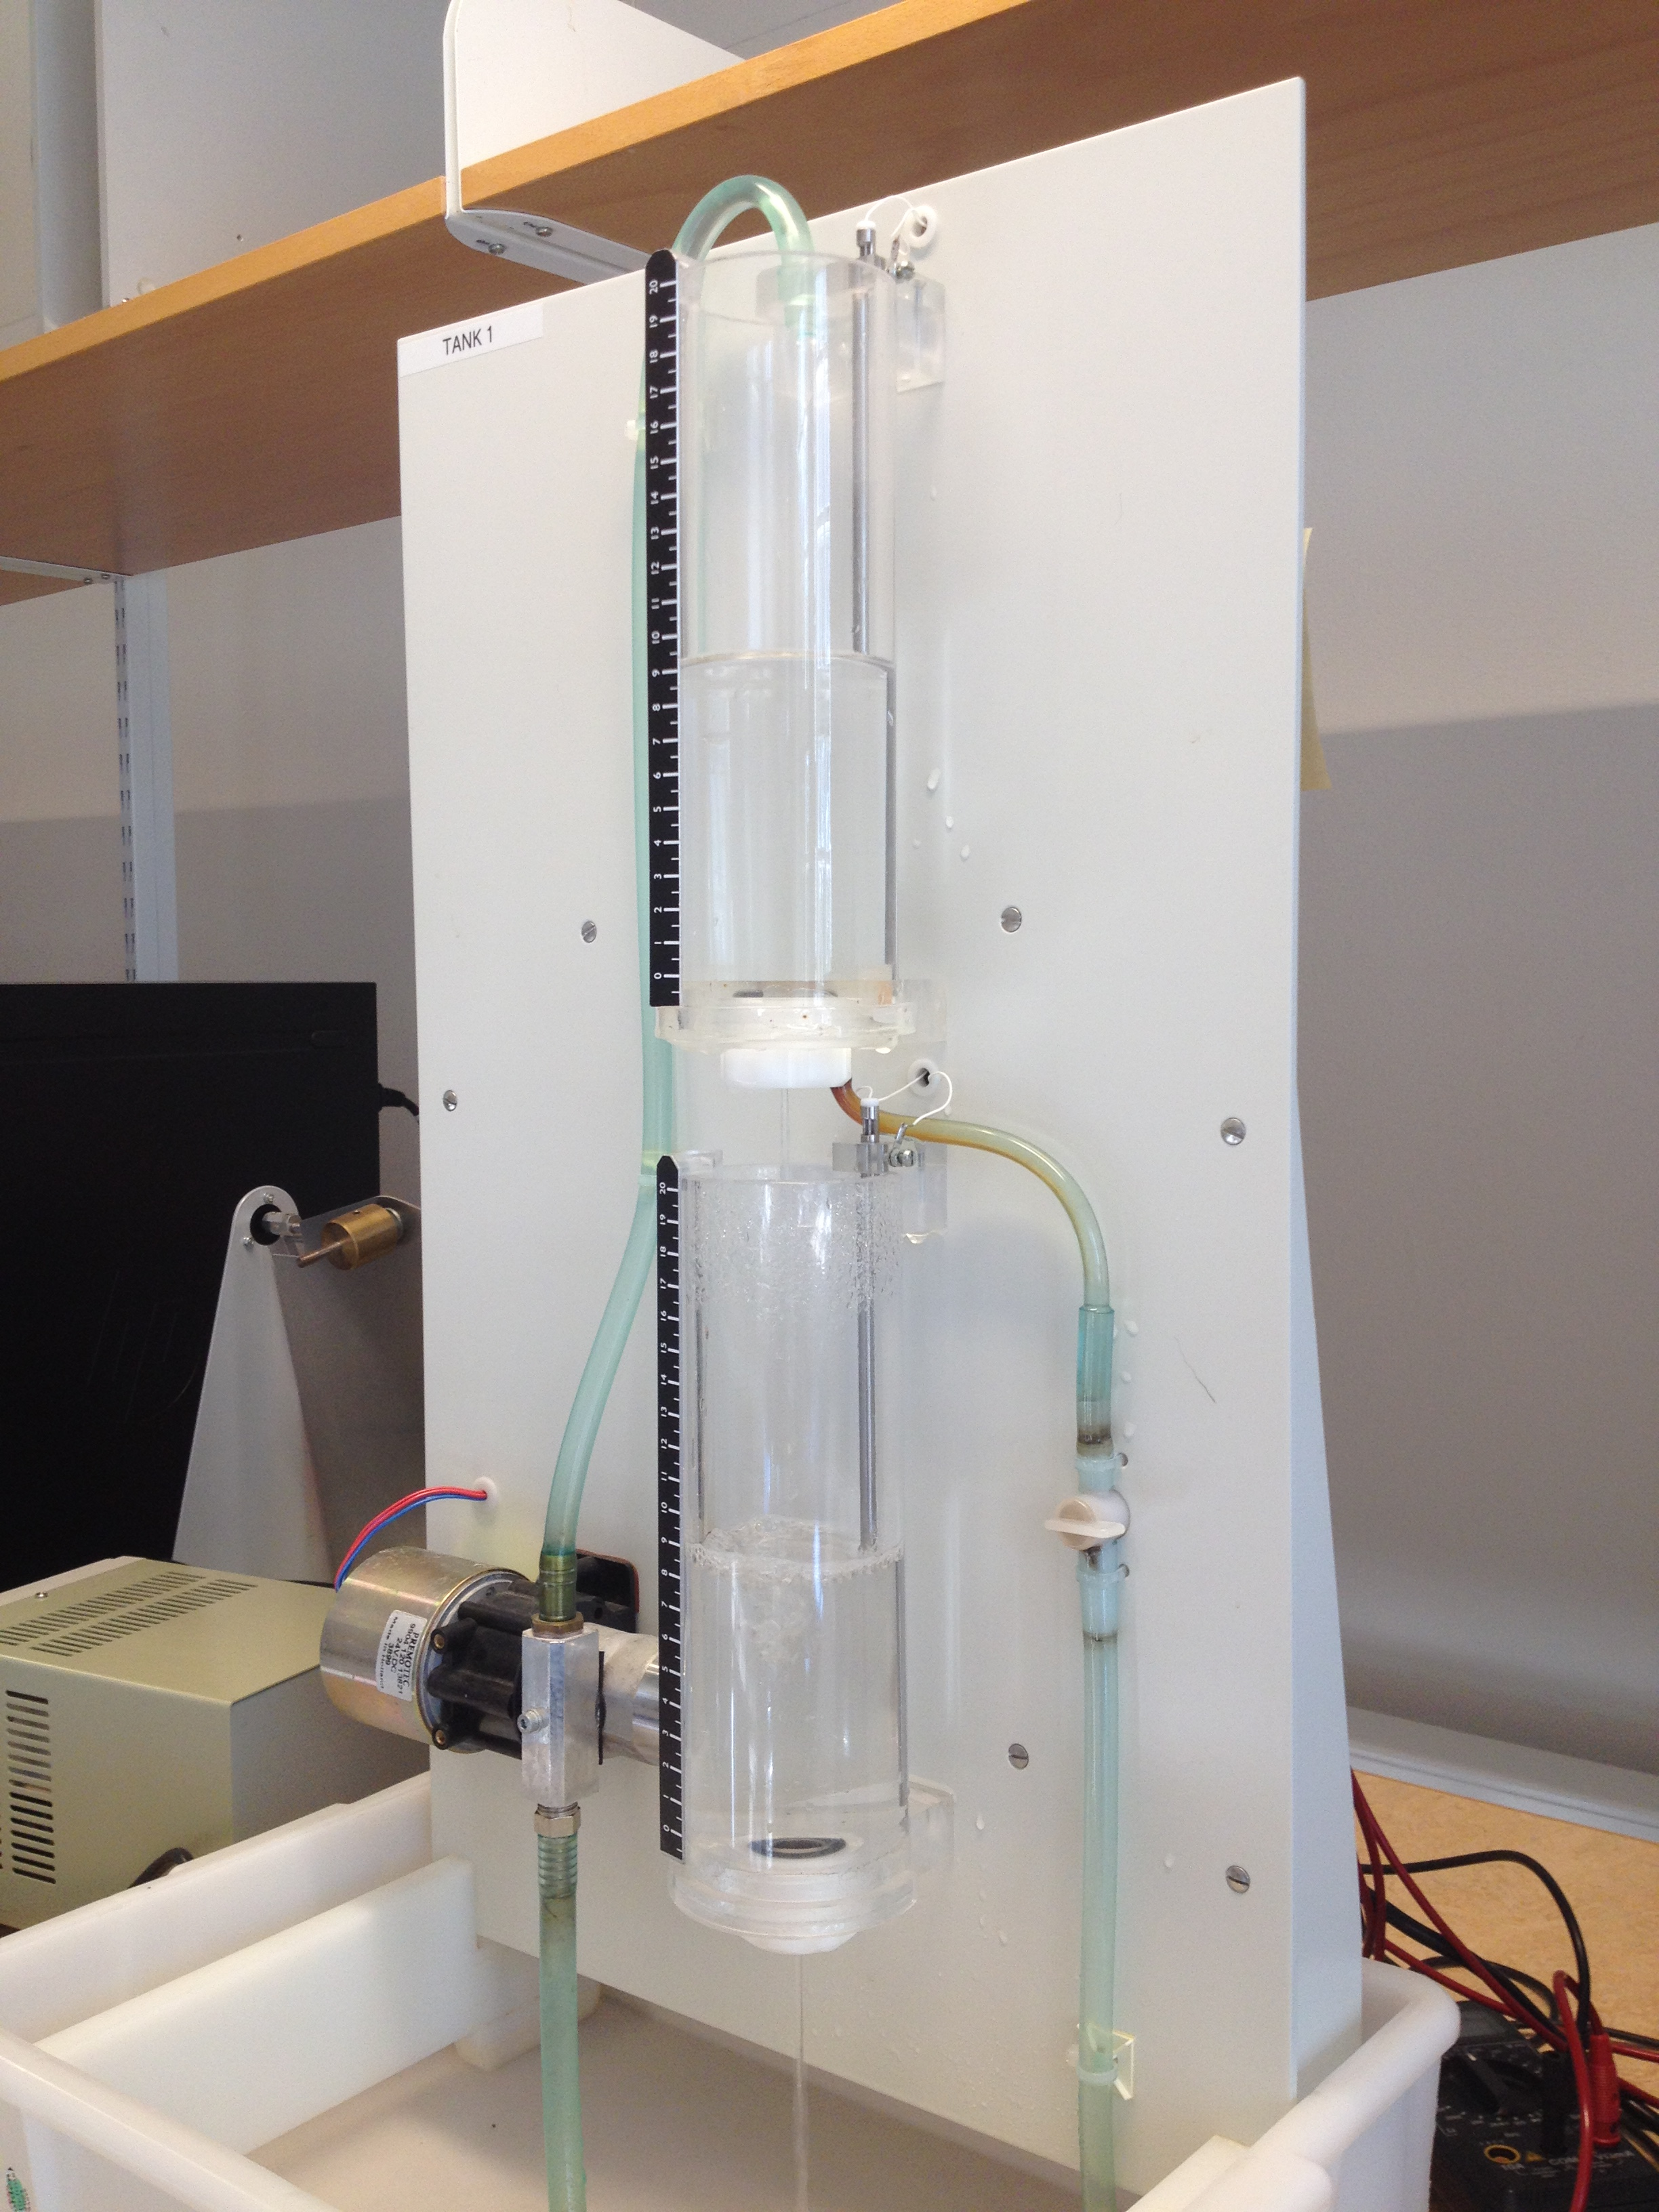
\includegraphics[width=.38\linewidth]{img/CTS/CTS.jpg}
\end{figure}
 \column{.4\textwidth}
\begin{figure}
\centering
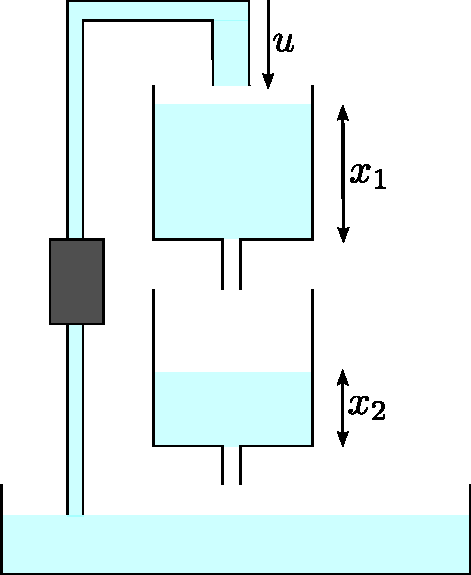
\includegraphics[width=.6\linewidth]{img/CTS/CTS_scheme.pdf}
\end{figure}
\end{columns}
\vskip .5em
%\pause
 Neural model structure: \structure{physics-inspired}
 \vskip -1.45em
\begin{align*}
 \dot x_1 &= \NN_{1}(x_1, u)\\
 \dot x_2 &= \NN_{2}(x_1, x_2, \alert{u})\\
 y        &= x_2
\end{align*}
\vskip -.5em
The dependency of $\NN_2$ on $u$ models \structure{water overflow} from upper tank.
%We could embed more insight (e.g., state $x_1$ does not depend on $x_2$\dots)
%Identification and validation datasets with $N=1024$ samples
\end{frame}

\begin{frame}{Numerical example}{Cascaded Tank System}
Training with $m=128, q=64$. Results on:% the ident/test datasets.\\
%Train time: 183~s
\vskip 1em
\begin{columns}
  \column{.5\textwidth}
  \centering
  Training dataset
  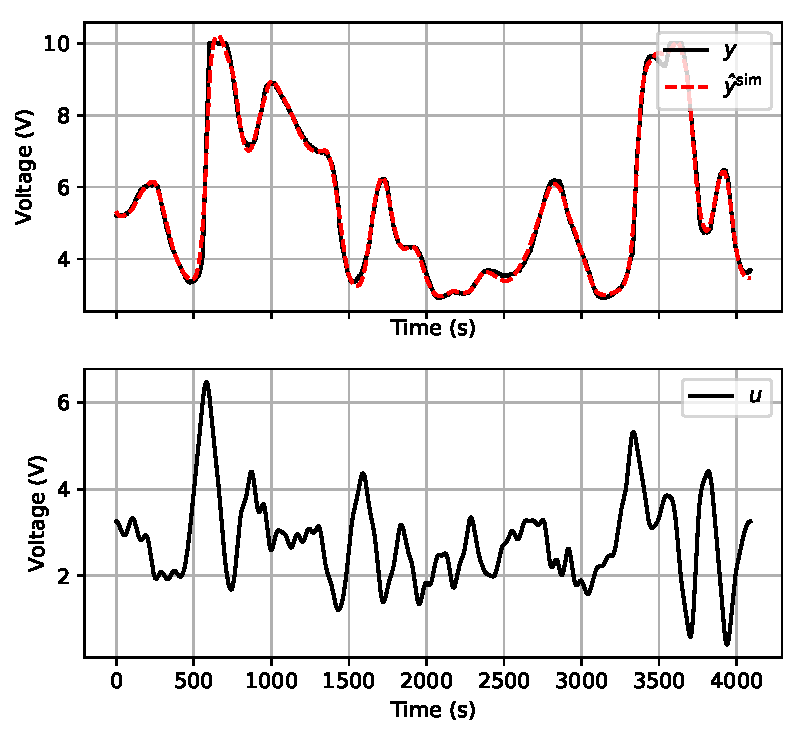
\includegraphics[width=\textwidth]{img/CTS/CTS_SS_id_model_SS_256step.pdf}
  $R^2 = 0.99$,\;$\text{RMSE}=0.08~\text{V}$
  \column{.5\textwidth}
    \centering
  Test dataset
  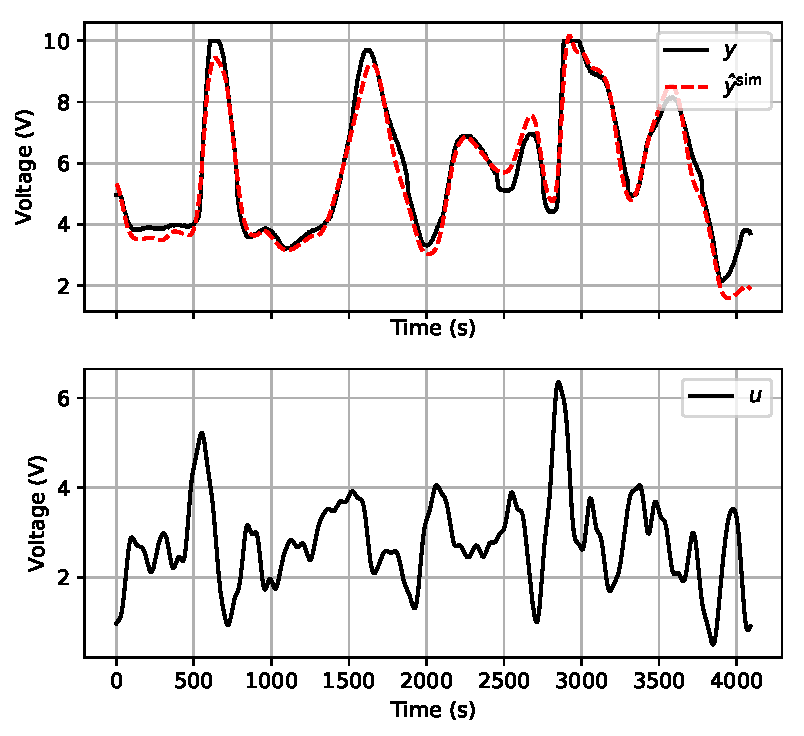
\includegraphics[width=\textwidth]{img/CTS/CTS_SS_val_model_SS_256step.pdf}
  $R^2 = 0.97$,\;$\text{RMSE}=0.33~\text{V}$
  \end{columns}
\end{frame}

% \begin{frame}{Simulation example}{Cascaded Tank System}
% 1024-step refining. Results \structure{in simulation} on the ident/val datasets.
% \vskip 1em
% \begin{columns}
%   \column{.5\textwidth}
%   \centering
%   Identification dataset
%   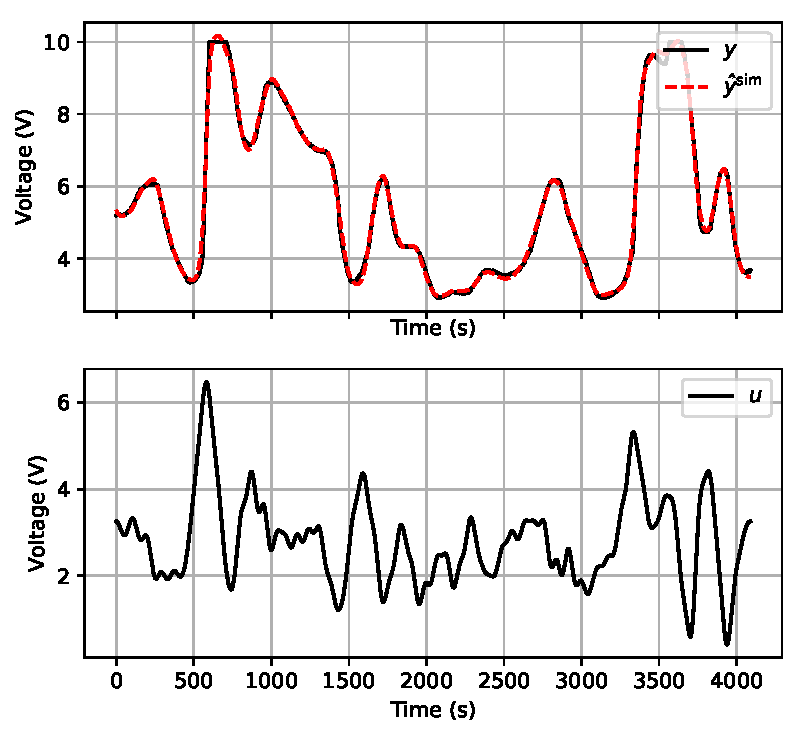
\includegraphics[width=\textwidth]{img/CTS/CTS_SS_id_model_SS_1024step.pdf}
%   $R^2 = 0.99$,\;$\text{RMSE}=0.12~\text{V}$
%   \column{.5\textwidth}
%     \centering
%   Validation dataset
%   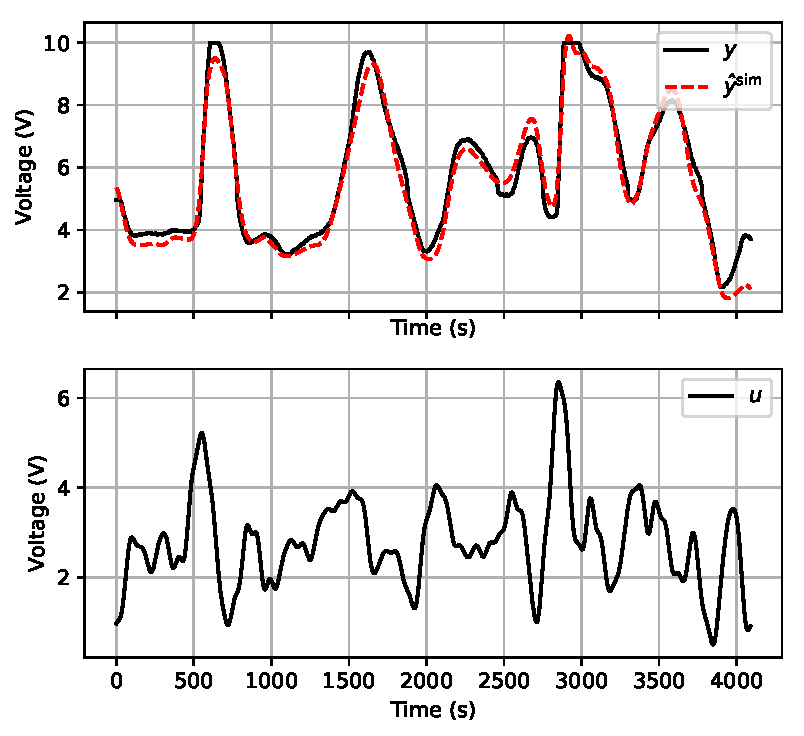
\includegraphics[width=\textwidth]{img/CTS/CTS_SS_val_model_SS_1024step.pdf}
%   $R^2 = 0.96$,\;$\text{RMSE}=0.42~\text{V}$
%   \end{columns}
% \end{frame}

\begin{frame}{Conclusions}{}
We have presented \structure{tailor-made} neural structures for system identification embedding a priori knowledge.
\vskip 1em
We have shown how to parallelize the training using batches of short-size \structure{subsequences}, and taking into account the effect of the \structure{initial condition}.
\pause
\vskip 1em
Current/Future work
\begin{itemize}
 \item Extension to the continuous-time setting
 \item Learning of Partial Differential Equations
\end{itemize}

\end{frame}


\begin{frame}{}{}
\begin{center}
\huge{\structure{Thank you.\\ Questions?}}
\vskip 1em
\begin{small}
\texttt{marco.forgione@idsia.ch}
\end{small}
\end{center}
\end{frame}

\end{document}

\end{document}
